% =====================================================================
\chapter{Método numérico}\label{cap:numerico}
% =====================================================================

La función de transferencia \eqref{eq:H} es exacta para campos continuos e infinitos. En la
computadora el campo se representa con un número finito de muestras y la transformada de
Fourier se sustituye por la transformada discreta (DFT), calculada con el algoritmo FFT
\parencite{cooley1965}. Este capítulo analiza qué condiciones deben cumplirse para que esa
sustitución no introduzca errores, y valida el propagador resultante. El artículo de
\textcite{chen2021} no describe su discretización.

\section{Discretización del campo}\label{sec:discretizacion}

Cada capa se representa con una malla de $\sqrt N\times\sqrt N$ muestras de paso
$\Delta x=d_f$: una muestra por neurona. Esta elección es coherente con la
\cref{sec:neurona}: la malla representa exactamente la banda $|u|\le1/(2d_f)$ que la red puede
controlar. Con la DFT sobre una ventana de $N_p$ muestras por lado, las frecuencias
disponibles son
\begin{equation}
  u_m=m\,\Delta u,\qquad \Delta u=\frac{1}{N_p\,\Delta x},\qquad
  m=-\tfrac{N_p}{2},\dots,\tfrac{N_p}{2}-1 ,
  \label{eq:frecuencias}
\end{equation}
y la propagación \eqref{eq:asm} se calcula como
\begin{equation}
  Y^{l+1}=\mathrm{recorte}\Bigl\{\mathrm{IFFT}\bigl[\mathrm{FFT}\{\mathrm{relleno}(Y^l\circ t^l)\}\cdot H(u_m,v_{m'};D)\bigr]\Bigr\}.
  \label{eq:asm-discreto}
\end{equation}

\section{Convolución circular y relleno con ceros}\label{sec:relleno}

La DFT trata el campo como si fuera periódico con periodo $N_p\Delta x$. Por eso el producto
en frecuencia de \eqref{eq:asm-discreto} equivale a una convolución \emph{circular}: la luz
que sale por un borde de la ventana reaparece por el opuesto. Para evitarlo, la capa de
$\sqrt N$ muestras se coloca en el centro de una ventana de $N_p=2\sqrt N$ muestras rellena de
ceros (\cref{fig:ventana}), y tras la propagación se conserva sólo la región central. El
recorte tiene además un significado físico: cada capa tiene tamaño finito $w$, y la luz que
cae fuera de ella se pierde.

\begin{figure}[htb]
\centering
\begin{tikzpicture}[x=1cm,y=1cm,>={Stealth[length=2mm]}]
  % ventana
  \fill[gray!8] (0,0) rectangle (8,4);
  \draw[gray,thick,dashed] (0,0) rectangle (8,4);
  \node[gray,font=\small,rotate=90] at (1.0,2.0) {ceros};
  \node[gray,font=\small,rotate=90] at (7.0,3.0) {ceros};
  % capa
  \fill[udlap!25] (2,0) rectangle (6,4);
  \draw[udlaposcuro,thick] (2,0) rectangle (6,4);
  \node[udlaposcuro,font=\small] at (4,3.6) {capa, $w=\sqrt N d_f$};
  % rayo
  \fill[udlaposcuro] (2.05,1.0) circle (2pt);
  \draw[->,very thick,azulfig] (2.05,1.0) -- (6.0,2.6) node[pos=0.55,above,sloped,font=\small] {onda plana de frecuencia $u$};
  \draw[->,very thick,red!70!black,dashed] (2.05,1.0) -- (8.0,1.6) ;
  \node[red!70!black,font=\small,align=left,anchor=west] at (8.1,1.6) {sale de la ventana:\\ reaparecería por la izquierda};
  % desplazamiento
  \draw[<->] (2.05,-0.35) -- (6.0,-0.35) node[midway,below,font=\small] {$z\tan\theta\le w$};
  \draw[<->] (0,4.35) -- (8,4.35) node[midway,above,font=\small] {ventana de cómputo: $N_p\Delta x=2w$};
\end{tikzpicture}
\caption[Ventana de cómputo y límite de banda]{Ventana de cómputo. La capa ocupa la mitad
central de una ventana rellena de ceros. Una onda plana con $\tan\theta=\lambda u/\sqrt{1-\lambda^2u^2}$ se
desplaza lateralmente $z\tan\theta$; si ese desplazamiento supera $w$, la convolución circular
la haría reaparecer por el borde opuesto (aliasing).}
\label{fig:ventana}
\end{figure}

\section{Muestreo de la función de transferencia}\label{sec:aliasing}

El relleno no basta. $H$ es una exponencial compleja cuya fase,
$\psi(u)=2\pi z\sqrt{1/\lambda^2-u^2-v^2}$, oscila cada vez más rápido al crecer $u$ y $z$. Si
cambia más de $\pi$ entre dos frecuencias consecutivas de \eqref{eq:frecuencias}, $H$ queda
submuestreada \parencite{voelz2009}. La ``frecuencia local'' de $H$ (en unidades de
longitud) es
\begin{equation}
  \frac{1}{2\pi}\left|\frac{\partial\psi}{\partial u}\right|
  =\frac{z\,|u|}{\sqrt{1/\lambda^2-u^2-v^2}} ,
  \label{eq:frec-local}
\end{equation}
y el criterio de Nyquist en el dominio de frecuencias exige que no supere $1/(2\Delta u)$.
Tomando $v=0$ y despejando:
\begin{align}
  \frac{z\,|u|}{\sqrt{1/\lambda^2-u^2}}\le\frac{1}{2\Delta u}
  \quad&\Longleftrightarrow\quad
  u^2\Bigl[(2\Delta u\,z)^2+1\Bigr]\le\frac{1}{\lambda^2}\nonumber\\
  &\Longleftrightarrow\quad
  |u|\le\flim\equiv\frac{1}{\lambda\sqrt{(2\Delta u\,z)^2+1}} .
  \label{eq:flim}
\end{align}
Éste es el límite de banda de \textcite{matsushima2009}: el \emph{espectro angular de banda
limitada} usa $H$ sólo para $|u|,|v|\le\flim$ y la anula fuera de esa banda.

\paragraph{Interpretación geométrica.} Con $\sin\theta=\lambda u$, el lado izquierdo de
\eqref{eq:flim} es $z\tan\theta$, y con $N_p=2\sqrt N$ se tiene $1/(2\Delta u)=N_p\Delta x/2=w$. El
límite de banda, por lo tanto, elimina exactamente las ondas planas cuyo desplazamiento
lateral $z\tan\theta$ supera $w$ (\cref{fig:ventana}): las que habrían dado la vuelta a la
ventana. Esas ondas tampoco habrían llegado a la capa siguiente, así que eliminarlas es
físicamente correcto.

\section{Distancia crítica}\label{sec:zc}

El método \emph{sin} límite de banda (``ingenuo'') es correcto mientras $\flim$ sea mayor que
la frecuencia de Nyquist de la malla, $1/(2\Delta x)$, porque entonces ninguna frecuencia
representable viola \eqref{eq:flim}. Imponiendo $\flim\ge1/(2\Delta x)$:
\begin{equation}
  (2\Delta u\,z)^2+1\le\frac{4\Delta x^2}{\lambda^2}
  \quad\Longrightarrow\quad
  z\le z_c\equiv\frac{N_p\Delta x}{2}\sqrt{\frac{4\Delta x^2}{\lambda^2}-1}
  \;\approx\;\frac{N_p\,\Delta x^2}{\lambda}.
  \label{eq:zc}
\end{equation}

\begin{calculo}[Distancia crítica en el sistema del artículo]
Con $N_p=2000$ y $\Delta x=\SI{4}{\micro m}$, la forma paraxial de \eqref{eq:zc} da
\[
  z_c\approx\frac{(2000)(\num{4e-6})^2}{\num{632.8e-9}}=\SI{50.6}{mm},
\]
y la forma exacta, $(\SI{4}{mm})\sqrt{158.8}=\SI{50.4}{mm}$. La separación del artículo
($D\approx\SI{50}{mm}$) cae justo en la frontera, de modo que el método ingenuo no es seguro;
por eso este trabajo usa el de banda limitada.
\end{calculo}

\section{El criterio de conectividad es la condición de muestreo}\label{sec:identidad}

Comparando \eqref{eq:zc} con \eqref{eq:dmin} aparece la misma expresión.

\begin{proposicion}\label{prop:identidad}
Si la malla tiene una muestra por neurona ($\Delta x=d_f$) y se rellena al doble
($N_p=2\sqrt N$), la distancia mínima de conectividad de \textcite{chen2021} coincide
exactamente con la distancia crítica del espectro angular:
\[
  \Dmin=z_c .
\]
Equivalentemente, en $z=\Dmin$ el límite de banda \eqref{eq:flim} es igual a la frecuencia de
Nyquist de la malla: $\flim(\Dmin)\cdot2d_f=1$.
\end{proposicion}

\begin{proof}
Con $\Delta x=d_f$ y $N_p=2\sqrt N$, $N_p\Delta x/2=\sqrt N d_f$, y \eqref{eq:zc} se convierte en
$z_c=\sqrt N d_f\sqrt{4d_f^2/\lambda^2-1}$, que es \eqref{eq:dmin}.
\end{proof}

\noindent La proposición no es una coincidencia: ambos criterios expresan la condición
$z\tan\varphi\le w$ para la onda plana más inclinada que representa la malla
(\cref{fig:cono,fig:ventana}). El cono de difracción de \textcite{chen2021} es,
literalmente, la condición de muestreo del propagador. Se verificó numéricamente para 15
combinaciones de $\sqrt N\in\{80,200,1000\}$ y $d_f/\lambda\in\{0.6,1,2,6,12\}$: en todas,
$\flim(\Dmin)\cdot2d_f=1.000000$ \parencite{repo2026}.

\section{Precisión numérica y costo computacional}\label{sec:costo}

\paragraph{Precisión.} En el sistema completo, la fase de $H$ llega a
$kD=2\pi(\SI{0.05}{m})/(\SI{632.8}{nm})\approx\num{4.96e5}$~rad. En precisión simple (32 bits)
los números de esa magnitud están espaciados \SI{0.031}{rad}, un error apreciable. Por eso
$H$ se calcula en doble precisión y sólo después se convierte a precisión simple.

\paragraph{Costo.} Una propagación son dos FFT bidimensionales de $N_p\times N_p$, con costo
$\mathcal{O}(N_p^2\log N_p)$. El sistema completo requiere $L+1=6$ propagaciones por imagen
hacia adelante y otras tantas hacia atrás (\cref{fig:adjunto}), sobre mallas de
$2000\times2000$. Cada campo complejo en precisión simple ocupa
$2000^2\times\SI{8}{B}=\SI{32}{MB}$; contando los campos intermedios que guarda la
diferenciación automática, se estima del orden de \SI{1}{GB} por imagen. Entrenar con
\num{80000} imágenes durante 20 épocas implica $1.6\times10^6$ pasos hacia adelante y hacia
atrás, lo que hace necesaria una GPU.

\section{Validación del propagador}\label{sec:validacion}

El propagador se comparó con tres referencias independientes (\cref{tab:validacion}).

\begin{table}[htb]
\centering
\caption{Validación del espectro angular de banda limitada.}
\label{tab:validacion}
\begin{tabularx}{\textwidth}{@{}>{\raggedright}p{4.6cm}X>{\raggedleft\arraybackslash}p{2.6cm}@{}}
\toprule
Prueba & Referencia & Error relativo máx.\\
\midrule
Apertura cuadrada de \SI{200}{\micro m}, $z=\SI{8}{mm}$ ($N_F\approx2$) &
Solución analítica de Fresnel con integrales de Fresnel \parencite[sec.~4.5]{goodman2005} &
\SI{0.04}{\percent}\\
Apertura circular de radio \SI{40}{\micro m}, campo en el eje &
Solución exacta de Rayleigh--Sommerfeld, $U=e^{\jj kz}-\frac{z}{R}e^{\jj kR}$ &
\SI{3.6}{\percent} ($z\ge\SI{0.3}{mm}$)\\
Capa con fase aleatoria, neuronas de \SI{4}{\micro m}, $z/z_c\in[1,20]$ &
Integral de Rayleigh--Sommerfeld \eqref{eq:rs} por suma directa &
\SIrange{3.5}{9.1}{\percent}\\
\bottomrule
\end{tabularx}
\end{table}

\begin{figure}[htb]
\centering
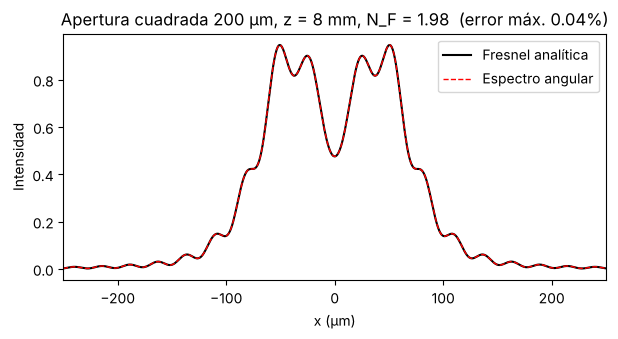
\includegraphics[width=0.85\textwidth]{b_apertura_cuadrada_fresnel.png}
\caption[Validación: apertura cuadrada]{Perfil de intensidad de una apertura cuadrada de
\SI{200}{\micro m} a \SI{8}{mm}: solución analítica de Fresnel y espectro angular.}
\label{fig:val-cuadrada}
\end{figure}

\begin{figure}[htb]
\centering
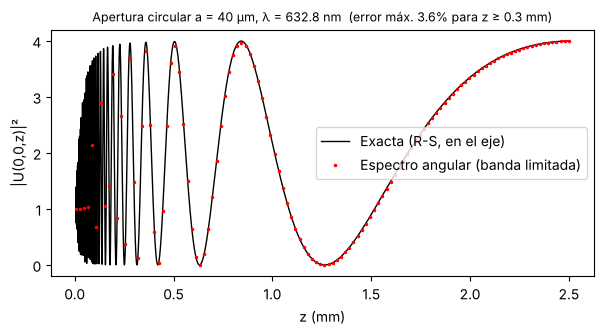
\includegraphics[width=0.85\textwidth]{a_apertura_circular.png}
\caption[Validación: apertura circular]{Intensidad en el eje de una apertura circular. Para
$z<\SI{0.3}{mm}$ el borde escalonado de un círculo pixelado cambia la fase de la onda de
borde, y las oscilaciones rápidas dejan de coincidir; no es un error del propagador sino de
la representación del círculo.}
\label{fig:val-circular}
\end{figure}

\begin{figure}[htb]
\centering
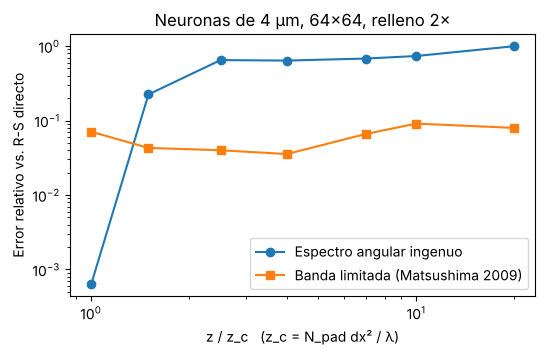
\includegraphics[width=0.7\textwidth]{c_aliasing_asm.png}
\caption[Validación: aliasing del espectro angular]{Error frente a la integral de
Rayleigh--Sommerfeld directa en función de $z/z_c$. El método ingenuo es exacto en $z=z_c$,
pero su error sube al 22--99\,\% en cuanto $z>z_c$; con límite de banda el error se mantiene
por debajo del 10\,\%. La comparación empieza en $z=z_c$ porque la suma directa sólo está
bien muestreada para $z\gtrsim z_c/2$, el régimen complementario.}
\label{fig:val-aliasing}
\end{figure}

\noindent El error residual del método de banda limitada (unos pocos por ciento) corresponde a
la luz que realmente sale de la ventana; la suma directa la cuenta y el propagador la
descarta. Para la red, cuyas capas son finitas, esa luz se perdería de todas formas.
